\documentclass[12pt,a4paper]{article}
\usepackage[utf8]{inputenc}
\usepackage{graphicx}
\usepackage{color}
\usepackage[magyar]{babel}
\usepackage{listings}
\usepackage{float}

\usepackage{enumerate}
\usepackage{tikz}
\usetikzlibrary{shapes,arrows}
\usetikzlibrary{positioning}
\usetikzlibrary{arrows.meta}

\tikzset{
block/.style = {draw, fill=white, rectangle, minimum height=3em, minimum width=3em},
tmp/.style  = {coordinate}, 
input/.style = {coordinate},
output/.style= {coordinate},
pinstyle/.style = {pin edge={to-,thin,black}
}
}
\usepackage[siunitx]{circuitikz} 
\renewcommand{\lstlistingname}{Lista}
\usepackage{hyperref}
\hypersetup{
	pdftitle={HA5KFU tanfolyam - Szoftverrádió gyakorlat},
	pdfauthor={HA5KFU Rádióamatőr Klub},
	pdfsubject={HA5KFU tanfolyam},
	pdfcreator={latex},
	pdfkeywords={ },
	pdfpagemode=UseOutlines,
	pdfdisplaydoctitle=true,
	pdflang=hu,
	unicode
}
\usepackage{color} %red, green, blue, yellow, cyan, magenta, black, white
\usepackage{xcolor}
\usepackage{textcomp}

\definecolor{comment}{RGB}{0,128,0} % dark green
\definecolor{string}{RGB}{255,0,0}  % red
\definecolor{keyword}{RGB}{0,0,255} % blue

\lstset{
	basicstyle=\footnotesize\ttfamily\color{black},
	commentstyle=\color{comment},
	stringstyle=\color{string},
	keywordstyle=\color{keyword},
	basicstyle=\footnotesize\ttfamily,
	numbers=left,
	numberstyle=\tiny,
	numbersep=5pt,
	frame=lines,
	breaklines=true,
	prebreak=\raisebox{0ex}[0ex][0ex]{\ensuremath{\hookleftarrow}},
	showstringspaces=false,
	upquote=true,
	tabsize=2,
}
\pagestyle{plain}
\sloppy
\begin{document}
\begin{center}

\includegraphics[width=300pt,keepaspectratio]{figures/ha5kfu.eps}
\\[0.5cm]
Rádióamatőr tanfolyamot segítő jegyzet, egyelőre kidolgozás alatt \\
Szabó Áron HA1FLX, HA5KFU... % Feel free to add yourself
\\[1cm]

{\huge \bfseries Szoftverrádió gyakorlat \\[2cm]}



\end{center}

\renewcommand{\contentsname}{Tartalom}\tableofcontents 
\newpage

\newpage

\section{Bevezető}
A gyakorlat célja a szoftverrádió lehetőségeinek megismerése, és bemutatása egy C nyelven megírt FM demodulátoron keresztül.

\section{Előkészületek}
A gyakorlathoz Linux operációs rendszerre lesz szükség.

\paragraph{Szükséges csomagok:} 
\begin{itemize}
	\item netcat
	\item rtl-sdr \textit{(saját Realtek alapú szoftverrádiós eszköz esetén)}
	\item tcc
	\item sox
	\item aplay
	\item \textit{ízlés szerinti szövegszerkesztő program }

\end{itemize}


\section{Elméleti összefoglaló}


\subsection{IQ demodulátorok}
Az IQ demodulátornál egy szinusz és egy koszinusz jellel is megszorozzuk a bejövő jelünket. A szinusznak és a koszinusznak a frekvenciája megegyezik. Feltételezve, hogy a felső keverési termékeket külön-külön kiszűrjük, megkapjuk a visszalassítós keverést. Az I és Q jelet lehet külön-külön digitalizálni, ezen a ponton már nem is szükséges nagyon gyors analógból digitális átalakítás, hiszen lassú jelekkel dolgozunk. Az I és Q jelek mint koordináták fogják megmutatni, hogy épp merre mutat a vett jel vektora, plusz a való életben valamekkora zaj is fog megjelenni ezen túl. Az IQ jelek digitálisan feldolgozhatóak, elvégezhető a demoduláció. Ezen az elven alapszik a gyakran használt RTL-SDR működése is, amivel például a SMOG jeleit is lehet fogni.

\clearpage
\section{Feladatok}

\subsection{IQ demodulátor}



\begin{figure}[H]
\label{fig:iq}
\centering
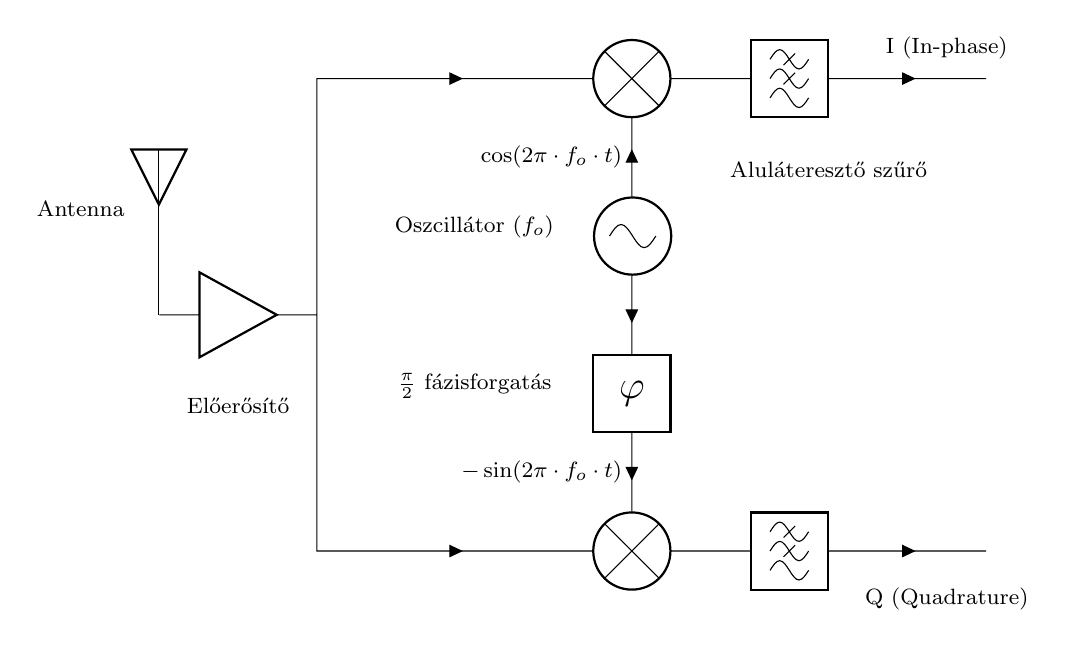
\begin{tikzpicture}

	\draw
	(-1,-2) node[label={[font=\footnotesize]above:Antenna}] {}
	(1,-4.5) node[label={[font=\footnotesize]above:Előerősítő}] {}
	(4,-1.5) node[label={[font=\footnotesize]below:Oszcillátor ($f_o$)}] {}
	(4,-3.5) node[label={[font=\footnotesize]below:$\frac{\pi}{2}$ fázisforgatás}] {}
	
	(8.5,-1.5) node[label={[font=\footnotesize]above:Aluláteresztő szűrő}] {}
	(10,0) node[label={[font=\footnotesize]above:I (In-phase)}] {}
	(10,-7) node[label={[font=\footnotesize]above:Q (Quadrature)}] {}
	
	%(0, -3) to [short] ++(1,0) 
	(2,-3) to [short] ++(0,3) to [short, i=\phantom{}] ++(3.5,0) 
	(2,-3) to [short] ++(0,-3) to [short, i=\phantom{}] ++(3.5,0) 	
	
	(6,-1.5) to [short, i=\footnotesize $\cos(2\pi \cdot f_o \cdot t)$] (6,-0.5)
	
	(6,-2.5) to [short, i=\phantom{}] (6,-3.5)
	
	(6,-4.5) to [short, i>_=\footnotesize $-\sin(2\pi \cdot f_o \cdot t)$] (6,-5.5)
	
	(6.5,0) to [short] ++(1,0) to [lowpass] ++(1,0) to [short, i=\phantom{}] ++(2,0) 
	(6.5,-6) to [short] ++(1,0) to [lowpass] ++(1,0) to [short, i=\phantom{}] ++(2,0) 
	(0, -3) to [amp] ++(2,0) 
	(6,0)[mixer] node(mixa){}	
	(6,-6)[mixer] node(mixb){}	
	

	(0,-3)[antenna]node(ant){}
	(6.5,-2)[oscillator] node(osc){}	
	(6,-4)[phaseshiftershape] node(phas){}	
	
	
	;
    \end{tikzpicture}
\caption{
Az IQ demodulátor blokkvázlata} 
\end{figure}


\begin{lstlisting}[frame=single,language=c,caption=Kiinduló kód]
#include <math.h>
#include <stdio.h>

int main()
{
	double i, q, s;
	for(;;)
	{
		i=((unsigned char)getchar()-127); 
		q=((unsigned char)getchar()-127);
		
		// s = ??;

		putchar((unsigned char)(s+127));
	}
}
\end{lstlisting}

\end{document}



